\documentclass[dvipsnames, aspectratio=169]{beamer}
\usepackage[utf8]{inputenc}
\usepackage{listings}
\usepackage{comment}
\usepackage{soul}
%\usepackage{ulem}
\usepackage{subfig}
\usepackage{pgf-pie}
\setul{}{1pt}
\usepackage[oldenum, olditem]{paralist}
%allow even smaller text
\newcommand\tinytiny{\fontsize{4pt}{3}\selectfont}

\makeatletter
\let\old@lstKV@SwitchCases\lstKV@SwitchCases
\def\lstKV@SwitchCases#1#2#3{}
\makeatother
\usepackage{lstlinebgrd}
\makeatletter
\let\lstKV@SwitchCases\old@lstKV@SwitchCases

\lst@Key{numbers}{none}{%
    \def\lst@PlaceNumber{\lst@linebgrd}%
    \lstKV@SwitchCases{#1}%
    {none:\\%
     left:\def\lst@PlaceNumber{\llap{\normalfont
                \lst@numberstyle{\thelstnumber}\kern\lst@numbersep}\lst@linebgrd}\\%
     right:\def\lst@PlaceNumber{\rlap{\normalfont
                \kern\linewidth \kern\lst@numbersep
                \lst@numberstyle{\thelstnumber}}\lst@linebgrd}%
    }{\PackageError{Listings}{Numbers #1 unknown}\@ehc}}
\makeatother


\usepackage{tikz}
\graphicspath{{3_7/figures/}}
%disclaimer for Sandia. uncomment and the whole blob goes away @ b80c116300122
\def\sandid{UPDATEME SAND2020-7755 PE}

% \title{Performance Portability with Kokkos}
\title{Kokkos 3.7 Release Briefing}

%BAD misuse of author field
\author{New Capabilities}


\usetheme{kokkos}

\newif\ifshort
\newif\ifmedium
\newif\iffull
\newif\ifnotoverview

\newcommand{\TutorialDirectory}{\texttt{Intro-Full}}
\newcommand{\ExerciseDirectory}[1]{\texttt{Exercises/#1/}}
\newcommand{\TutorialClone}{\texttt{Kokkos/kokkos-tutorials/\TutorialDirectory}}

\definecolor{darkgreen}{rgb}{0.0, 0.5, 0.0}
\definecolor{darkred}{rgb}{0.8, 0.0, 0.0}
\definecolor{orange}{rgb}{0.8, 0.33, 0.0}
\definecolor{purple}{rgb}{0.60, 0.20, 0.80}
\colorlet{bodyColor}{blue!20}
\colorlet{patternColor}{orange!30}
\colorlet{policyColor}{green!30}

% http://tex.stackexchange.com/questions/144448/color-a-text-line-in-a-code-lstlisting
\lstnewenvironment{code}[1][]%
{
  %with txfonts: OT1/txr/m/n/10
  %with default fonts: OT1/cmr/m/n/10
  %\fontfamily{cmr}\selectfont
  %\showthe\font
   \noindent
   \minipage{\linewidth}
   %\vspace{0.5\baselineskip}
   \lstset{mathescape, escapeinside={<@}{@>},
moredelim=**[is][{\btHL[fill=patternColor]}]{@pattern}{@pattern},
moredelim=**[is][{\btHL[fill=red!30]}]{@warning}{@warning},
moredelim=**[is][{\btHL[fill=policyColor]}]{@policy}{@policy},
moredelim=**[is][{\btHL[fill=bodyColor]}]{@body}{@body},
moredelim=**[is][{\btHL[fill=red!30]}]{@warning}{@warning},
moredelim=**[is][\color{black}]{@black}{@black},
moredelim=**[is][\color{blue}]{@blue}{@blue},
moredelim=**[is][\bf]{@bold}{@bold},
moredelim=**[is][\it]{@italic}{@italic},
moredelim=**[is][\color{boldblue}\bf]{@boldblue}{@boldblue},
moredelim=**[is][\color{red}]{@red}{@red},
moredelim=**[is][\color{green}]{@green}{@green},
moredelim=**[is][\color{gray}]{@gray}{@gray},
moredelim=**[is][\color{darkgreen}]{@darkgreen}{@darkgreen},
moredelim=**[is][\color{darkred}]{@darkred}{@darkred},
moredelim=**[is][\color{orange}]{@orange}{@orange},
moredelim=**[is][\color{purple}]{@purple}{@purple},
keywords={},
#1}
}
{
  \endminipage
  %\vspace{1.0\baselineskip}
}

\makeatletter
\newif\ifATOlinebackground
\lst@Key{linebackground}{\tiny}{\def\ATOlinebackground{#1}\global\ATOlinebackgroundtrue}
\makeatother

\lstnewenvironment{shell}[1][]{%
  \global\ATOlinebackgroundfalse
  \lstset{language=sh,%
    showstringspaces=false,
    aboveskip=0pt,
    frame=none,
    numbers=none,
    belowskip=2pt,
    breaklines=true,
    #1,
    }
  %\ifATOlinebackground
  \lstset{linebackgroundcolor={
    \ATOlinebackground
  }}
  %\fi
  }{}

\lstnewenvironment{cmake}[1][]{%
  \global\ATOlinebackgroundfalse
  \lstset{language=sh,%
    showstringspaces=false,
    aboveskip=0pt,
    frame=none,
    numbers=none,
    belowskip=2pt,
    breaklines=true,
    #1,
    }
  %\ifATOlinebackground
  \lstset{linebackgroundcolor={
    \ATOlinebackground
  }}
  %\fi
  }{}

\newcommand{\inlinecode}[1]{{\lstset{basicstyle=\ttfamily,keywordstyle={},showstringspaces=false}\lstinline$#1$}}
\newcommand{\inlineshell}[1]{{\lstset{basicstyle=\ttfamily,keywordstyle={},showstringspaces=false}\lstinline$#1$}}

\setbeamercolor{block title}{fg=white, bg=SandiaLightBlue}
\setbeamercolor{block body}{bg=lightgray}
\setbeamercolor{block title alerted}{fg=white, bg=SandiaRed}
\setbeamercolor{block body alerted}{bg=lightgray}



%\usepackage[texcoord,grid,gridunit=mm,gridcolor=red!10,subgridcolor=green!10]{eso-pic}
\usepackage[absolute,overlay]{textpos}





% http://tex.stackexchange.com/questions/8851/how-can-i-highlight-some-lines-from-source-code

\usepackage{pgf, pgffor}
\usepackage{listings}
\usepackage{lstlinebgrd} % see http://www.ctan.org/pkg/lstaddons

\makeatletter
%%%%%%%%%%%%%%%%%%%%%%%%%%%%%%%%%%%%%%%%%%%%%%%%%%%%%%%%%%%%%%%%%%%%%%%%%%%%%%
%
% \btIfInRange{number}{range list}{TRUE}{FALSE}
%
% Test in int number <number> is element of a (comma separated) list of ranges
% (such as: {1,3-5,7,10-12,14}) and processes <TRUE> or <FALSE> respectively

\newcount\bt@rangea
\newcount\bt@rangeb

\newcommand\btIfInRange[2]{%
    \global\let\bt@inrange\@secondoftwo%
    \edef\bt@rangelist{#2}%
    \foreach \range in \bt@rangelist {%
        \afterassignment\bt@getrangeb%
        \bt@rangea=0\range\relax%
        \pgfmathtruncatemacro\result{ ( #1 >= \bt@rangea) && (#1 <= \bt@rangeb) }%
        \ifnum\result=1\relax%
            \breakforeach%
            \global\let\bt@inrange\@firstoftwo%
        \fi%
    }%
    \bt@inrange%
}
\newcommand\bt@getrangeb{%
    \@ifnextchar\relax%
        {\bt@rangeb=\bt@rangea}%
        {\@getrangeb}%
}
\def\@getrangeb-#1\relax{%
    \ifx\relax#1\relax%
        \bt@rangeb=100000%   \maxdimen is too large for pgfmath
    \else%
        \bt@rangeb=#1\relax%
    \fi%
}

%%%%%%%%%%%%%%%%%%%%%%%%%%%%%%%%%%%%%%%%%%%%%%%%%%%%%%%%%%%%%%%%%%%%%%%%%%%%%%
%
% \btLstHL<overlay spec>{range list}
%
% TODO BUG: \btLstHL commands can not yet be accumulated if more than one overlay spec match.
%
\newcommand<>{\btLstHL}[2]{%
  \only#3{\btIfInRange{\value{lstnumber}}{#1}{\color{#2}\def\lst@linebgrdcmd{\color@block}}{\def\lst@linebgrdcmd####1####2####3{}}}%
}%
\makeatother






% http://tex.stackexchange.com/questions/15237/highlight-text-in-code-listing-while-also-keeping-syntax-highlighting
%\usepackage[T1]{fontenc}
%\usepackage{listings,xcolor,beramono}
\usepackage{tikz}

\makeatletter
\newenvironment{btHighlight}[1][]
{\begingroup\tikzset{bt@Highlight@par/.style={#1}}\begin{lrbox}{\@tempboxa}}
{\end{lrbox}\bt@HL@box[bt@Highlight@par]{\@tempboxa}\endgroup}

\newcommand\btHL[1][]{%
  \begin{btHighlight}[#1]\bgroup\aftergroup\bt@HL@endenv%
}
\def\bt@HL@endenv{%
  \end{btHighlight}%
  \egroup
}
\newcommand{\bt@HL@box}[2][]{%
  \tikz[#1]{%
    \pgfpathrectangle{\pgfpoint{1pt}{0pt}}{\pgfpoint{\wd #2}{\ht #2}}%
    \pgfusepath{use as bounding box}%
    \node[anchor=base west, fill=orange!30,outer sep=0pt,inner xsep=1pt, inner ysep=0pt, rounded corners=3pt, minimum height=\ht\strutbox+1pt,#1]{\raisebox{1pt}{\strut}\strut\usebox{#2}};
  }%
}
\makeatother



\usetikzlibrary{calc}
\usepackage{xparse}%  For \NewDocumentCommand

% tikzmark command, for shading over items
\newcommand{\tikzmark}[1]{\tikz[overlay,remember picture] \node (#1) {};}

\makeatletter
\NewDocumentCommand{\DrawBox}{s O{}}{%
    \tikz[overlay,remember picture]{
    \IfBooleanTF{#1}{%
        \coordinate (RightPoint) at ($(left |- right)+(\linewidth-\labelsep-\labelwidth,0.0)$);
    }{%
        \coordinate (RightPoint) at (right.east);
    }%
    \draw[red,#2]
      ($(left)+(-0.2em,0.9em)$) rectangle
      ($(RightPoint)+(0.2em,-0.3em)$);}
}

\NewDocumentCommand{\DrawBoxWide}{s O{}}{%
    \tikz[overlay,remember picture]{
    \IfBooleanTF{#1}{%
        \coordinate (RightPoint) at ($(left |- right)+(\linewidth-\labelsep-\labelwidth,0.0)$);
    }{%
        \coordinate (RightPoint) at (right.east);
    }%
    \draw[red,#2]
      ($(left)+(-\labelwidth,0.9em)$) rectangle
      ($(RightPoint)+(0.2em,-0.3em)$);}
}

\NewDocumentCommand{\DrawBoxWideBlack}{s O{}}{%
    \tikz[overlay,remember picture]{
    \IfBooleanTF{#1}{%
        \coordinate (RightPoint) at ($(left |- right)+(\linewidth-\labelsep-\labelwidth,0.0)$);
    }{%
        \coordinate (RightPoint) at (right.east);
    }%
    \draw[black,#2]
      ($(left)+(-\labelwidth,0.9em)$) rectangle
      ($(RightPoint)+(0.2em,-0.3em)$);}
}
\makeatother

\usetikzlibrary{positioning}

\usetikzlibrary{shapes}

\hypersetup{
    colorlinks=true,
    linkcolor=blue,
    filecolor=magenta,
    urlcolor=cyan,
}



\shorttrue
\mediumfalse
\fullfalse

\begin{document}

\begin{frame}
	\titlepage
\end{frame}


\begin{frame}[fragile]{Outline}

\textbf{3.7 Release Higlights}

    \begin{itemize}
      \item{Documentation}
      \item{SIMD}
      \item{HIPManagedSpace}
      \item{More View Allocation Properties Support}
      \item{Initialization}
      \item{Deprecations}
      \item{Kokkos 4.0 preview}
    \end{itemize}

\end{frame}

\begin{frame}{Find More}

\textbf{Online Resources}:

\begin{itemize}
        \item \url{https://github.com/kokkos}:
                \begin{itemize}
                        \item Primary Kokkos GitHub Organization
                \end{itemize}
        \item \url{https://github.com/kokkos/kokkos-tutorials/wiki/Kokkos-Lecture-Series}:
                \begin{itemize}
			\item{Slides, recording and Q\&A for the Full Lectures}
                \end{itemize}
        \item \url{https://kokkos.github.io/kokkos-core-wiki}:
                \begin{itemize}
                        \item Wiki including API reference
                \end{itemize}
        \item \url{https://kokkosteam.slack.com}:
                \begin{itemize}
                        \item Slack channel for Kokkos.
                        \item Please join: fastest way to get your questions answered.
                        \item Can whitelist domains, or invite individual people.
                \end{itemize}
\end{itemize}

\end{frame}

\begin{frame}[fragile]{Kokkos Usage}
  \textbf{Would like to strengthen community bonds and discoverability}

\vspace{10pt}
\textit{List of Applications and Libraries}
\begin{itemize}
\item Add your app to \url{https://github.com/kokkos/kokkos/issues/1950}
\item We are planning to add that to a Kokkos website.
\item Helps people discover each other when working on similar things.
\end{itemize}

\vspace{10pt}
\textit{GitHub Topics}
\begin{itemize}
\item Use \textit{kokkos} tag on your repos.
\item If you click on the topic you get a list of all projects on github with that topic.
\end{itemize}

\end{frame}

\begin{frame}[fragile]{Kokkos Topic}
  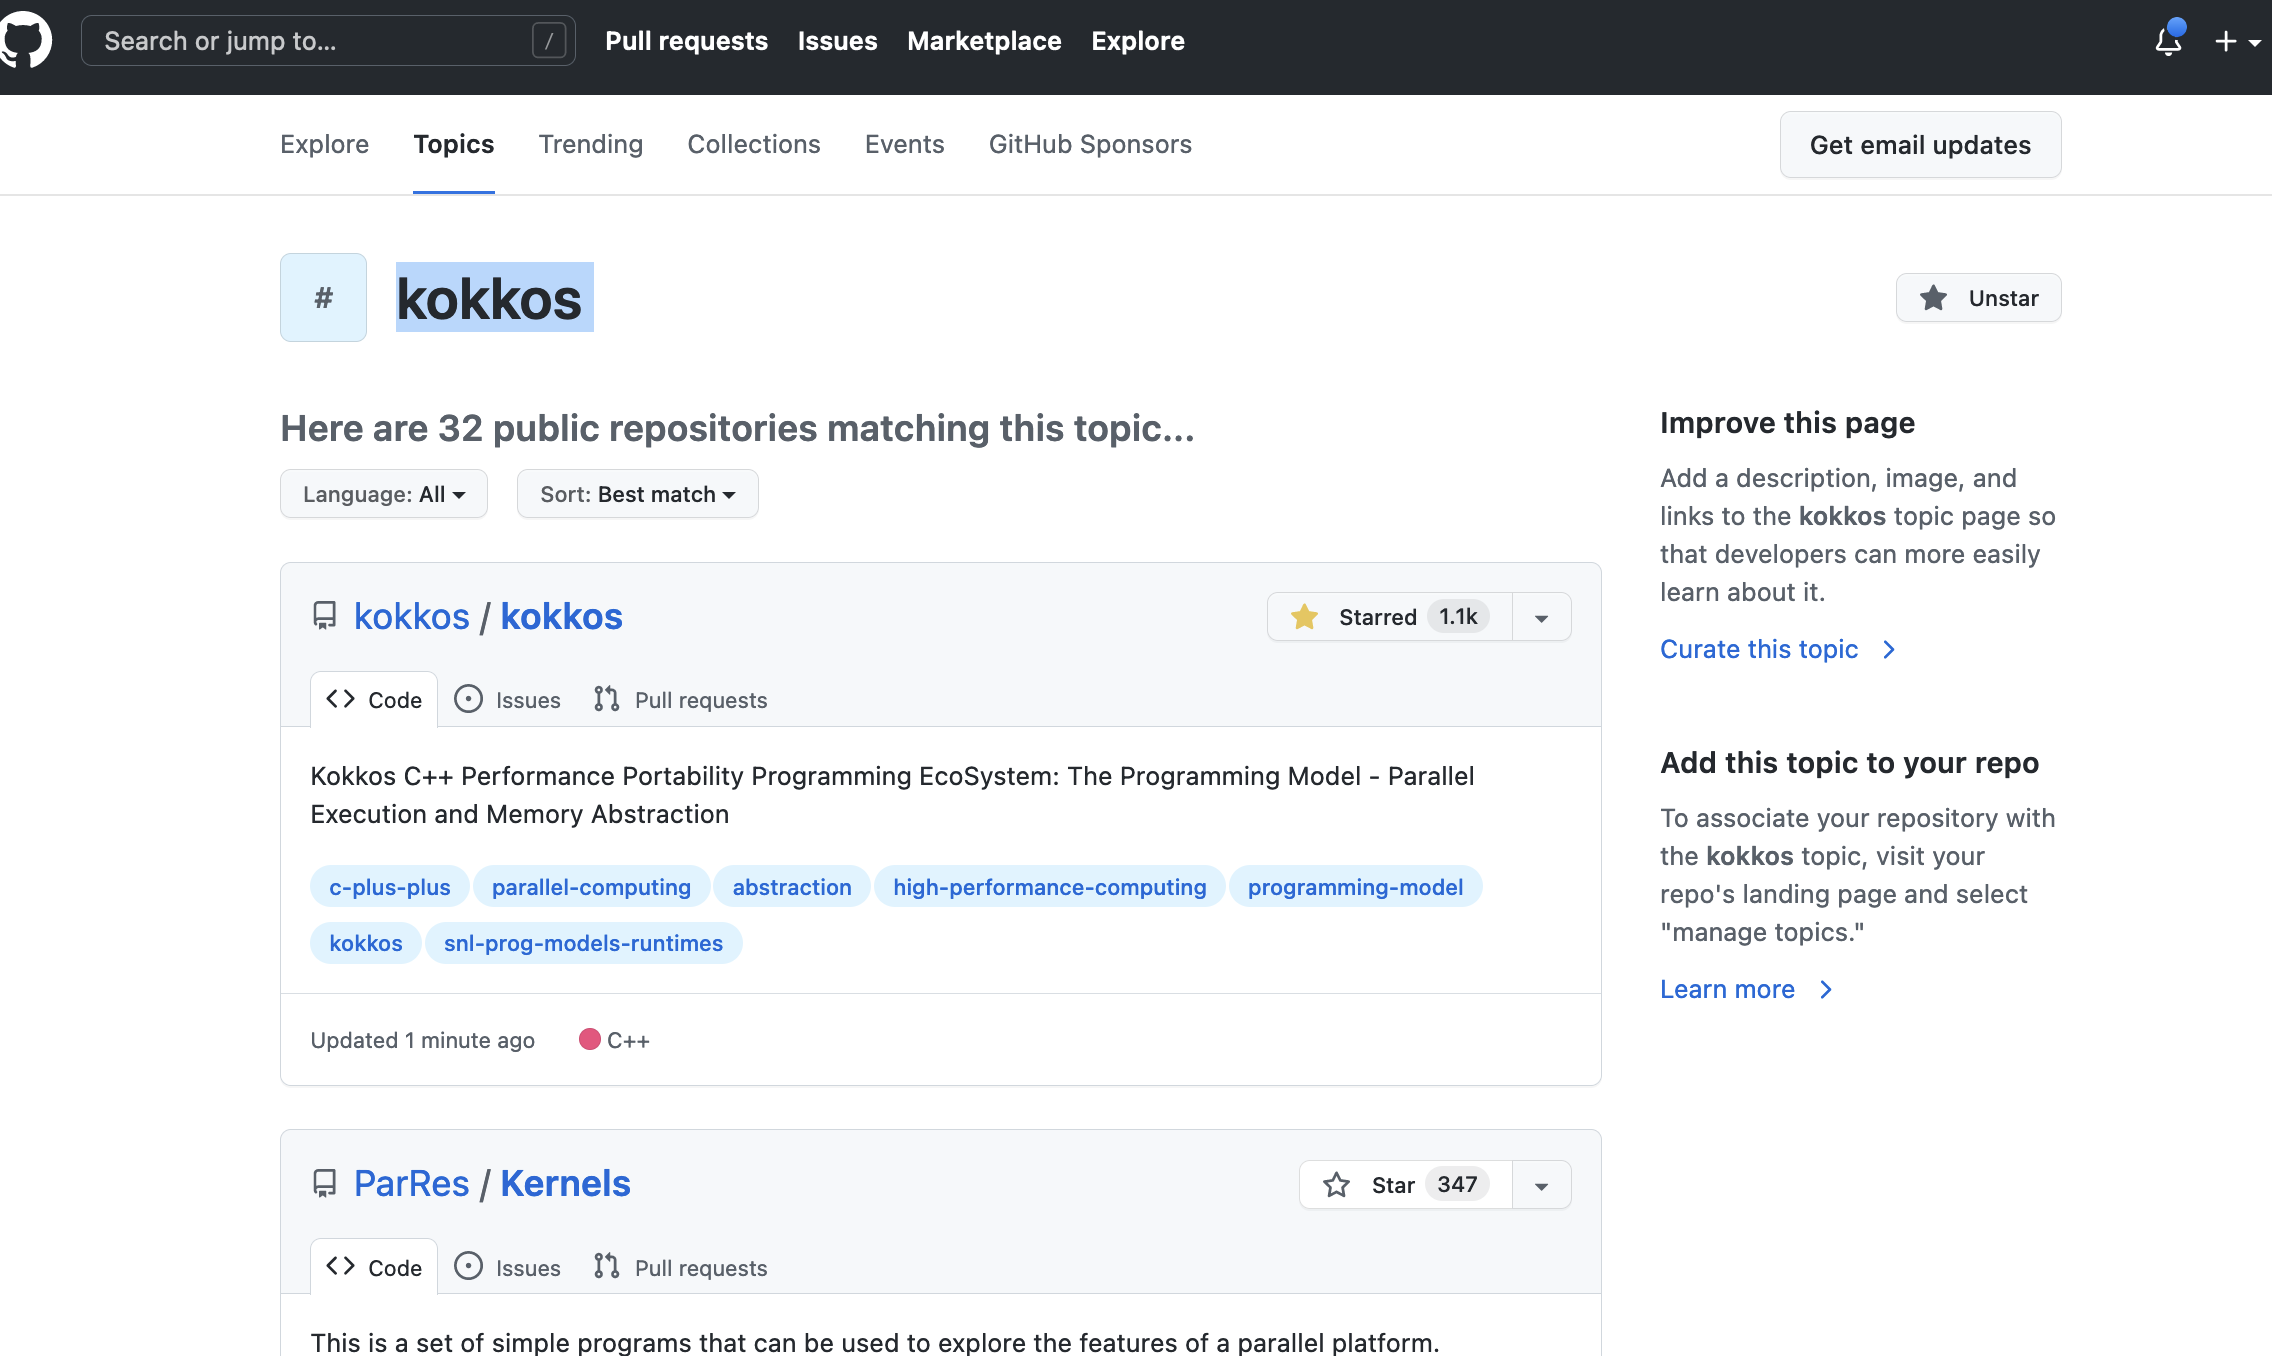
\includegraphics[width=0.9\textwidth]{3_7/kokkos-topic.png}
\end{frame}


%==========================================================================

\begin{frame}[fragile]

        {\Huge New Documentation Website}

  \vspace{-20pt}

\end{frame}

%==========================================================================

\begin{frame}[fragile]{Transition to github.io}
\textbf{Kokkos Documentation Now on \url{https://kokkos.github.io}}

\begin{itemize}
  \item {Transition to Sphinx syntax}
  \item {More flexibility in site layout and style}
  \item {Better update processes}
  \begin{itemize}
    \item {Source for core documentaiton at \url{https://github.com/kokkos/kokkos-core-wiki}}
    \item {Using pull requests with auto deploy}
    \item {Pull requests to improvde documentation are welcome!}
  \end{itemize}
\end{itemize}
\end{frame}

\begin{frame}[fragile]{Transition to github.io}
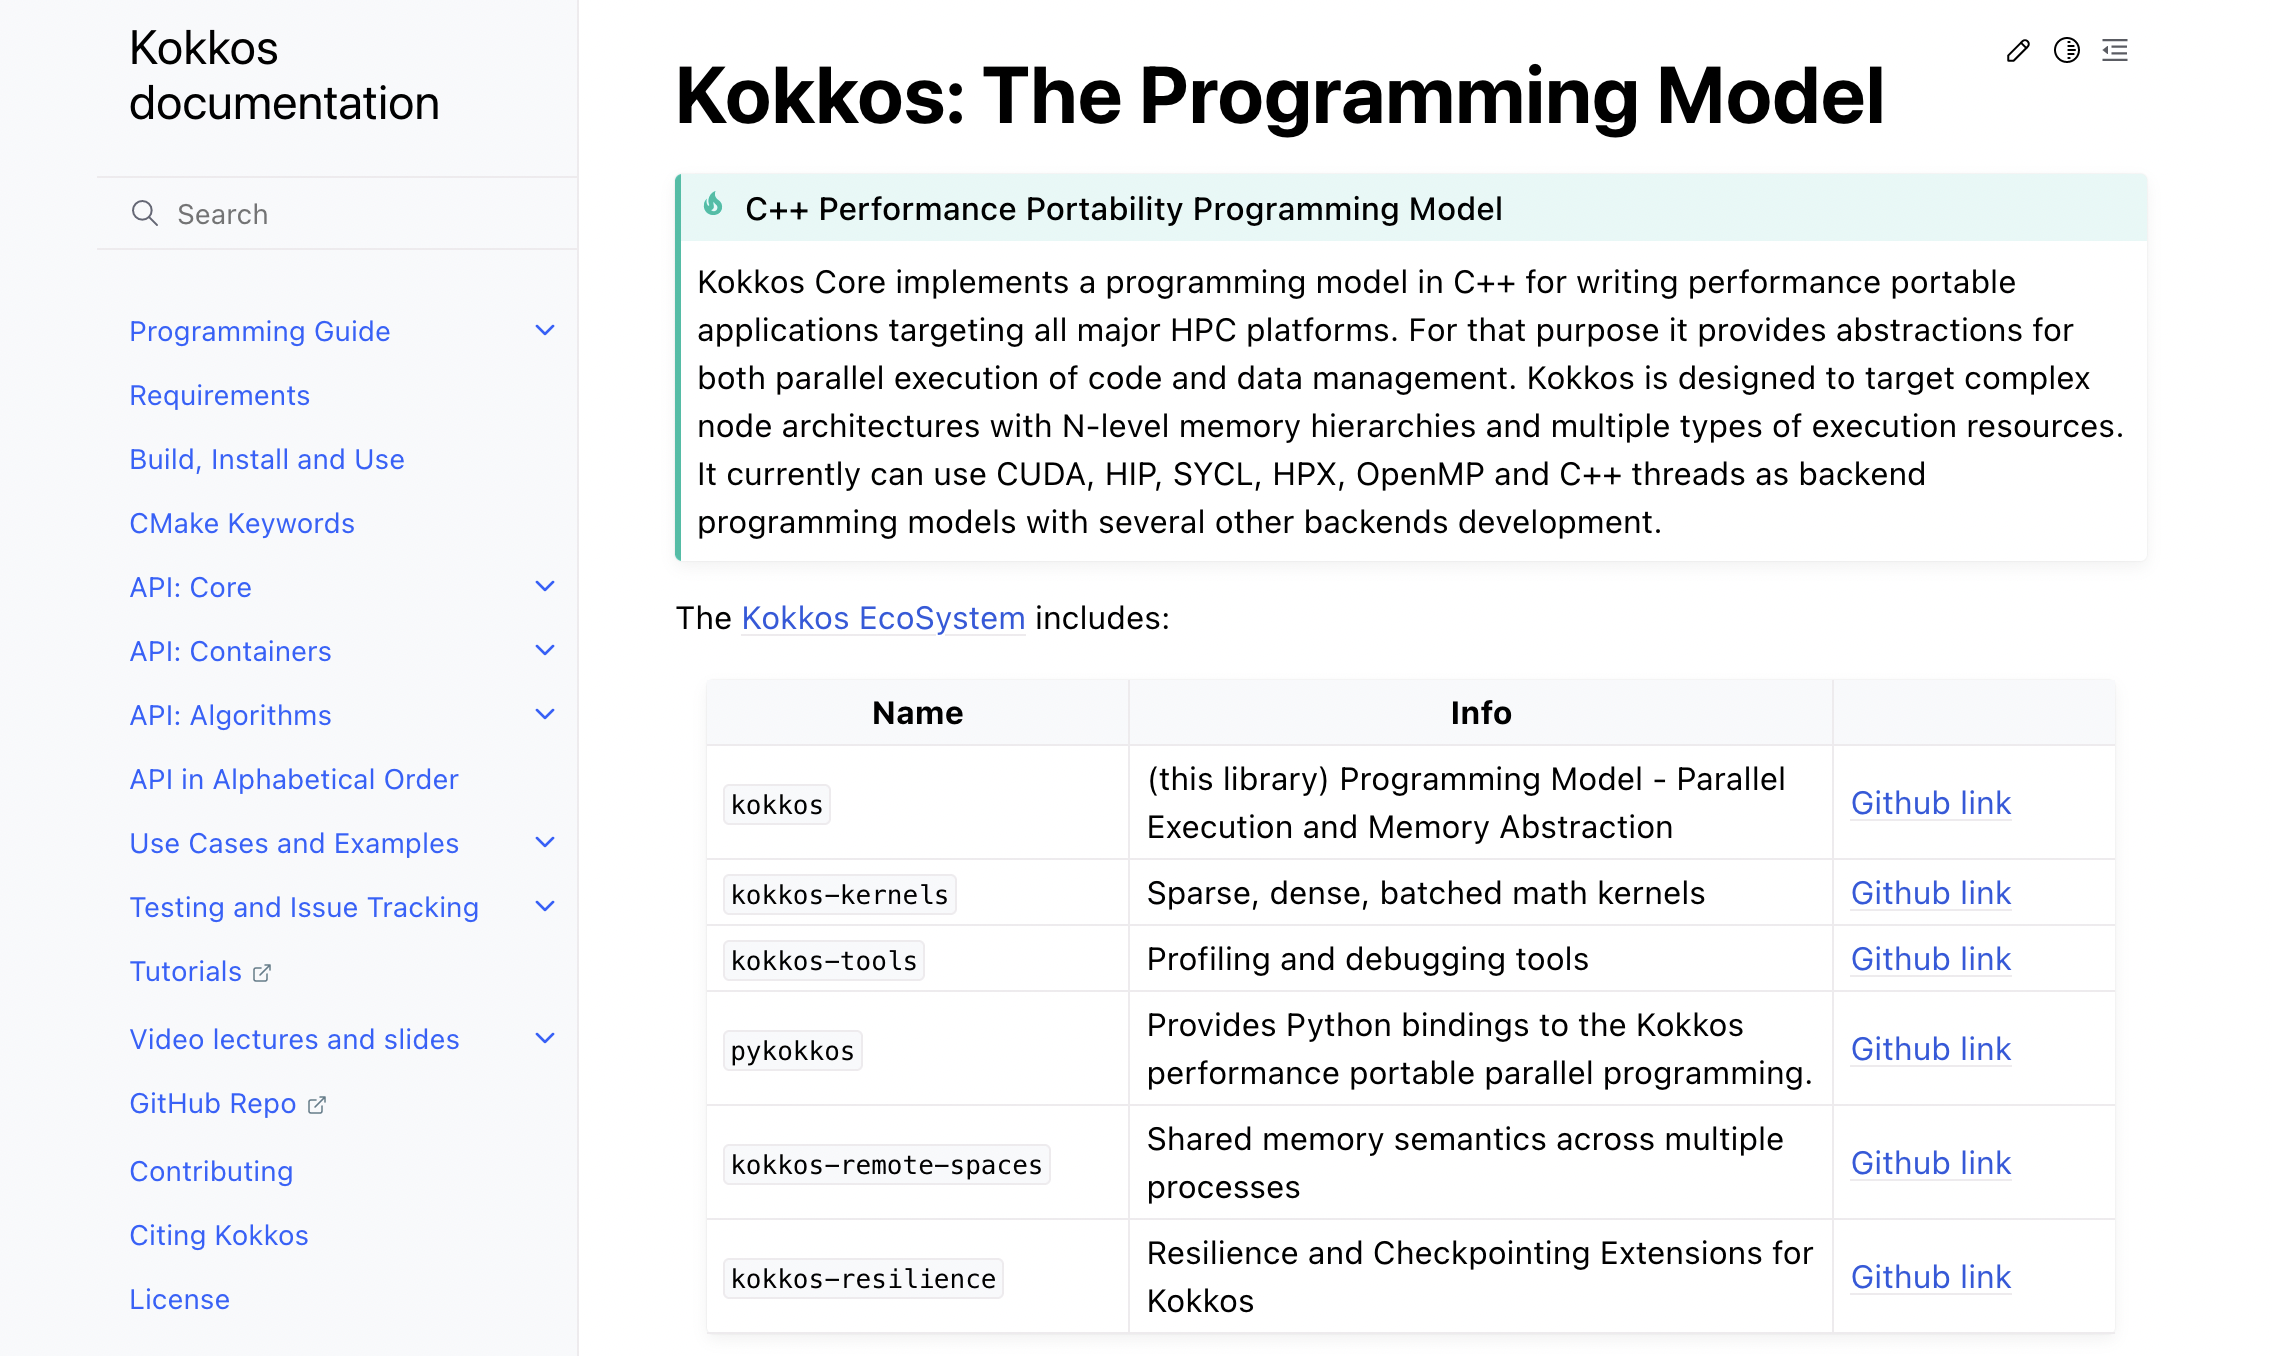
\includegraphics[width=0.9\textwidth]{3_7/website.png}
\end{frame}

\begin{frame}[fragile]{Good to know}
\textbf{Math functions are now in the primary namespace}
\begin{itemize}
  \item Now call \texttt{Kokkos::sin} etc. instead of \texttt{Kokkos::Experimental::sin}
\end{itemize}

\vspace{20pt}
\textbf{Enabled nested reduce with teams that are not power-of-two size!} 

\end{frame}


%==========================================================================

\begin{frame}[fragile]

  {\Huge SIMD}

  \vspace{10pt}

  {\large Portable vector intrinsic types.}

  \vspace{20pt}

  \textbf{Learning objectives:}
  \begin{itemize}
    \item {How to use SIMD types to improve vectorization.}
    \item {SIMD Types as an alternative to ThreadVector loops.}
    \item {SIMD Types to achieve outer loop vectorization.}
  \end{itemize}

  \vspace{-20pt}

\end{frame}

%==========================================================================

\begin{frame}[fragile]{Vectorization In Kokkos}

   So far there were two options for achieving vectorization: 

\begin{itemize}
  \item{{\textbf{Hope For The Best}}: Kokkos semantics make loops inherently vectorizable, sometimes the compiler figures it even out.}
  \item{{\textbf{Hierarchical Parallelism}}: {\texttt{TeamVectorRange}} and {\texttt{ThreadVectorRange}} help the compiler with hints such as {\texttt{\#pragma ivdep}} or {\texttt{\#pragma omp simd}}}.
\end{itemize}

   \vspace{3pt}

  These strategies do run into limits though:

\begin{itemize}
  \item{Compilers often do not vectorize loops on their own.}
  \item{An optimal vectorization strategy would require \emph{outer-loop vectorization}.}
  \item{Vectorization with \texttt{TeamVectorRange} sometimes requires artifically introducing an additional loop level.}
\end{itemize}
\end{frame}

\begin{frame}[fragile]{Outer-Loop Vectorization}

   A simple scenario where for outer-loop vectorization:
	\vspace{-3pt}
  \begin{code}[linebackgroundcolor={},keywords={for,int}]
  for(int i=0; i<N; i++) {
    // expect K to be small odd 1,3,5,7 for physics reasons
    for(int k=0; k<K; k++) b(i) += a(i,k);
  }
  \end{code}

  Vectorization the \texttt{K}-Loop is not profitable:
  \begin{itemize}
	  \item{It is a short reduction.}
	  \item{Remainders will eat up much time.}
  \end{itemize}
	\vspace{5pt}

  Using \texttt{ThreadVectorRange} is cumbersome and requires split of \texttt{N}-Loop:

  \begin{code}[linebackgroundcolor={},keywords={parallel_for,for,int,TeamPolicy,ThreadVectorRange}]
parallel_for("VectorLoop",TeamPolicy<>(0,N/V,V),
  KOKKOS_LAMBDA ( const team_t& team ) {
  int i = team.league_rank() * V;
  for(int k=0; k<K; k++) 
    parallel_for(ThreadVectorRange(team,V), [&](int ii) {
      b(i+ii) += a(i+ii,k);
    });
});
    \end{code}
\end{frame}

\begin{frame}[fragile]{SIMD Types}
  
   To help with this situation and (in particular in the past) fix the lack of auto-vectorizing compilers \texttt{SIMD-Types} have been invented. They:
	\begin{itemize}
		\item{Are short vectors of scalars.}
		\item{Have operators such as \texttt{+=} so one can use them like scalars.}
		\item{Are compile time sized.}
		\item{Usually map directly to hardware vector instructions.}
	\end{itemize}
	
	\begin{block}{Important concept: SIMD Type}
		A SIMD variable is a \textbf{short vector} which acts like a scalar.
  \end{block}

	Using such a \texttt{simd} type one can simply achieve \emph{outer-loop} vectorization by using arrays of \texttt{simd} and dividing the loop range by its \emph{size}.
\end{frame}

\begin{frame}[fragile]{Outer-Loop Vectorization}

  Lets take a look back at the outer loop vectorization:
  \begin{code}[linebackgroundcolor={},keywords={for,int}]
  View<double*> b = ...
  View<double**> a = ...
  for(int i=0; i<N; i++) {
    // expect K to be small odd 1,3,5,7 for physics reasons
    for(int k=0; k<K; k++) b(i) += a(i,k);
  }
  \end{code}

  \pause
  Using SIMD types is conceptionally as simple as:
	\begin{itemize}
		\item Replace scalar type with SIMD type
		\item Adjust loop iteration count by SIMD length
	\end{itemize}

  \begin{code}[linebackgroundcolor={},keywords={for,int}]
  using simd_t = Kokkos::Experimental::simd<double>;
  View<simd_t*> b = ...
  View<simd_t**> a = ...
  int V = simd_t::size();
  for(int i=0; i<N/V; i++) {
    // expect K to be small odd 1,3,5,7 for physics reasons
    for(int k=0; k<K; k++) b(i) += a(i,k);
  }
  \end{code}
\end{frame}

\begin{frame}[fragile]{C++26 SIMD}
	The ISO C++ standard has data-parallel types (\texttt{SIMD}) (in \emph{C++26}):

  \begin{code}[linebackgroundcolor={},keywords={template,class,public,using}]
template< class T, class Abi >
class basic_simd {
public:
  using value_type = T;
  using abi_type   = Abi;
  using mask_type  = basic_simd_mask<sizeof(T), Abi>;

  static constexpr integral_constant<simd-size-type, ...> size {};
  constexpr T operator[] (simd-size-type) const;
  // Element-wise operators
};

// Element-wise non-member functions

  \end{code}

\end{frame}

\begin{frame}[fragile]{C++26 SIMD ABI}
One interesting innovation here is the \texttt{Abi} parameter allowing for different, hardware specific, implementations.

	\vspace{8pt}

The most important components of \texttt{basic\_simd} are:
\begin{itemize}
	\item{\textbf{scalar\_abi}: single element type.}
	\item{\textbf{native\_abi}: best fit for hardware.}
	\item{\textbf{fixed\_size$<$N$>$}: the width of the simd type.}
\end{itemize}

\pause
	\vspace{8pt}

	But \texttt{std::simd} doesn't support GPUs ...

	\pause
	\vspace{8pt}
	It also has other problems making it insufficient for our codes...
\end{frame}

\begin{frame}[fragile]{Kokkos SIMD}
   Just at Sandia we had at least \textbf{5} different SIMD types in use.

   \vspace{8pt}
   A unification effort was started with the goal of:
   \begin{itemize}
      \item{Match the proposed \texttt{std::simd} API as far as possible.}
      \item{Support GPUs.}
      \item{Can be used stand-alone or in conjunction with Kokkos.}
      \item{Replaces all current implementations at Sandia for SIMD.}
   \end{itemize}

\end{frame}

\begin{frame}[fragile]{Kokkos SIMD}
  As with the C++26 SIMD type, it takes a data type and ABI
  \begin{code}
     template <class T, class Abi>
     class basic_simd;
  \end{code}

  Supported ABIs are:
  \begin{itemize}
    \item \texttt{simd\_abi::scalar}: a single element
    \item \texttt{simd\_abi::$[$native\_$]$fixed\_size<N>}: a specific data-parallel type available on the architecture (e.g. \texttt{avx512\_fixed\_size})
  \end{itemize}

  But for convenience, a simplified alias for \texttt{basic\_simd} is available:
  \begin{code}
    template <class T, int N = /* native_simd_width */>
    using simd = basic_simd<...>;
  \end{code}

  This abstracts ABI and allows using the optimal native data-parallel width on the architecture

\end{frame}

\begin{frame}[fragile]{Exercise: Simple SIMD usage.}

  \textbf{Details}:
  \begin{small}
  \begin{itemize}
\item Location: \ExerciseDirectory{simd/Begin}
\item Include the \texttt{Kokkos\_SIMD.hpp} header.
\item Change the data type of the views to use \texttt{simd$<$double$>$}.
\item Create an unmanaged \texttt{View$<$double*$>$} of \texttt{results} using the \texttt{data()} function for the final reduction.  
\end{itemize}
  \end{small}

\begin{code}
  # Configure, build, and run
    cmake -Bbuilddir -DKokkos_ARCH_NATIVE=ON
    cmake --build builddir
    ./builddir/SIMD
\end{code}

	\vspace{-3pt}
\ul{\textbf{Things to try:}}
  \begin{small}
  \begin{itemize}
  \item Vary problem size (-N ...; -M ...)
  \item Compare behavior of scalar vs vectorized on CPU and GPU
  \end{itemize}
  \end{small}



\end{frame}

\begin{comment}
\begin{frame}[fragile]{The GPU SIMD Problem}
  The above exercise used a \textbf{scalar} simd type on the \textbf{GPU}.
  
	{\textbf Why wouldn't we use a fixed\_size instead?}

	\begin{itemize}
	   \item{Using a \texttt{fixed\_size} ABI will create a scalar of size \texttt{N} in each CUDA thread!}
	   \item{Loading a \texttt{fixed\_size} variable from memory would result in uncoalesced access.}
           \item{If you have correct layouts you get \texttt{outer-loop} vectorization implicitly on GPUs.}
	\end{itemize}

	\pause
	But what if you really want to use \textbf{warp}-level parallelization for SIMD types?

	\pause
	{\textbf We need \emph{two} SIMD types: a \emph{storage} type and a \emph{temporary} type!}
\end{frame}

\begin{frame}[fragile]{cuda\_warp ABI}
  \begin{block}{Important concept: simd::storage\_type}
    Every \texttt{simd$<$T,ABI$>$} has an associated \texttt{storage\_type} typedef.
  \end{block}

  To help with the GPU issue we split types between \textbf{storage} types used for \texttt{Views}, and \textbf{temporary} variables.

  \begin{itemize}
	  \item{Most \texttt{simd::simd} types will just have the same \texttt{storage\_type}.}
	  \item{\texttt{simd$<$T,cuda\_warp$<$N$> >$} will use warp level parallelism.}
	  \item{\texttt{simd$<$T,cuda\_warp$<$N$> >$::storage\_type} is different though!}
	  \item{Used in conjunction with \texttt{TeamPolicy}.}
  \end{itemize}
\end{frame}

\begin{frame}[fragile]{cuda\_warp ABI}
\textbf{Illustrating difference between \texttt{pack} and \texttt{cuda\_warp}}


      \begin{code}[linebackgroundcolor={},keywords={simd,parallel_for,using}]
using ABI = ... ;
View<simd<double,ABI::storage_type> A(...);
parallel_for(TeamPolicy<>(N,AUTO,V), 
 KOKKOS_LAMBDA(const teamt_t& team) {
  int i = team.league_rank()*team.team_size()+team.team_rank();
  simd<double,ABI> tmp = A(i);
});
       \end{code}
  \begin{columns}[]
    \begin{column}{.5\textwidth}
      \begin{code}[linebackgroundcolor={},keywords={pack,using}]
using ABI = pack<8>; int V=1;
\end{code}

       \includegraphics[width=0.75\textwidth]{figures/simd-fixedsize} 

    \end{column}
    \begin{column}{.5\textwidth}
      \begin{code}[linebackgroundcolor={},keywords={cuda_warp,using}]
using ABI = cuda_warp<8>; int V=8;
\end{code}

       \includegraphics[width=0.75\textwidth]{figures/simd-warp} 

    \end{column}
  \end{columns}
\end{frame}

\begin{frame}[fragile]{cuda\_warp ABI}

Example of using \texttt{storage\_type}:

\begin{code}[linebackgroundcolor={},keywords={template,class,simd,simd_storage,TeamPolicy,TeamThreadRange,public,using}]
// Using cuda_warp abi
using simd_t = simd::simd<T,simd::simd_abi::cuda_warp<V> >;
// Define simd_storage type
using simd_storage_t = simd_t::storage_type;
// Allocate memory
View<simd_storage_t**> data("D",N,M); // will hold N*M*V Ts

// Launch Loop with vectorlength V
parallel_for("Loop", TeamPolicy<>(N,M,V), 
  KOKKOS_LAMBDA(const team_t& team) {
    int i = team.league_rank();
    parallel_for(TeamThreadRange(team,M), [&](int j) {
      // Load storage type into internal type;
      simd_t tmp = data(i,j);
      // Do something with it
      tmp *= 2.0;
      // write values back
      data(i,j) = tmp;
      // or inline:
      // data(i,j) = 2.0*simd_t(data(i,j));
  }); 
});
\end{code}

\end{frame}


\begin{frame}[fragile]{Exercise: SIMD storage usage.}

  \textbf{Details}:
  \begin{small}
  \begin{itemize}
\item Location: \ExerciseDirectory{simd\_warp/Begin}
\item Include the \texttt{simd.hpp} header.
\item Change the data type of the views to use \texttt{simd::simd$<$double,simd::simd\_abi:cuda\_warp$<32>>$::storage\_type}.
\item Create an unmanaged \texttt{View$<$double*$>$} of \texttt{results} using the \texttt{data()} function for the final reduction.  
\item Use inside of the lambda the \texttt{simd::simd$<$double,simd::simd\_abi:cuda\_warp$<32>>$} as scalar type.
\end{itemize}
  \end{small}

\begin{code}
   # Compile for GPU
   make -j KOKKOS_DEVICES=Cuda
   # Run on GPU
   ./simd.cuda
\end{code}

\end{frame}
\end{comment}

\begin{frame}[fragile]{Advanced SIMD Capabilities}

Kokkos SIMD supports math operations:
\begin{itemize}
  \item{Common stuff like \texttt{abs}, \texttt{sqrt}, \texttt{exp}, ...}
\end{itemize}

\vspace{8pt}
It also supports masking:

	\begin{code}
// Scalar code with condition:
for(int i=0; i<N; i++) {
  if( a(i) < 100.0 ) b(i) = a(i);
  else b(i) = 100.0;
}

// Becomes
using simd_t      = simd<double>;
using simd_mask_t = simd_t::mask_type;
   
for(int i=0; i<N/V; i++) {
  simd_t threshold(100.0), a_i(a_v(i));
  simd_mask_t is_smaller = threshold<a_i;

  b_v(i) = condition(is_smaller,a_i,threshold);
}
\end{code}
\end{frame}

\begin{frame}[fragile]{SIMD Summary}
	\begin{itemize}
		\item{SIMD types help vectorize code.}
		\item{In particular for \textbf{outer-loop} vectorization.}
		\item{There are \textbf{storage} and \textbf{temporary} types.}
		\item{Masking is supported too.}
	\end{itemize}
\end{frame}
%==========================================================================


%==========================================================================

\begin{frame}[fragile]

  {\Huge \texttt{HIP} MemorySpaces}

\end{frame}


%==========================================================================

\begin{frame}[fragile]{\texttt{HIPManagedSpace}}

  {\large \texttt{HIP} backend got a new page-migrating memory space}

  \vspace{20pt}

  \begin{itemize}
    \item Page migrating memory space similar to \texttt{CudaUVMSpace} for \texttt{HIP}
    \item Coarse-grained memory, thus changes are visible at kernel exit (also changed for \texttt{HIPHostPinnedSpace})
    \item OS migrates memory to local memory on access (\textbf{not} zero copy access like \texttt{HIPHostPinnedSpace})
  \end{itemize}

  \vspace{10pt}
  \textit{No configure time option to make it the default!}

\end{frame}

%==========================================================================

\begin{frame}[fragile]

  {\large Requirements for page-migration on \texttt{HIP}}

  \begin{itemize}
    \item Have a GPU that supports the feature (e.g. $\geq$ MI200)
    \item Have a OS that supports the feature (e.g. Kernel HMM module)
    \item Compile with \texttt{xnack:+} or \texttt{xnack:any} (default)
    \item Set runtime variable \texttt{HSA\_XNACK=1} or \texttt{amdgpu.noretry=0} at boot time
  \end{itemize}

  \vspace{10pt}
  \textbf{Without working xnack (compiletime and runtime) the memory will not migrate but be zero copy access via the interconnecting bus}

\end{frame}



%==========================================================================

\begin{frame}[fragile]

  {\Huge More View Allocation Properties Support}

  \vspace{10pt}

  \textbf{Content:}
  Support \texttt{view\_alloc} argument for
  \begin{itemize}
    \item \texttt{resize}
    \item \texttt{realloc}
    \item \texttt{create\_mirror}
    \item \texttt{create\_mirror\_view}
    \item \texttt{create\_mirror\_view\_and\_copy}
  \end{itemize}
  for \texttt{View}-like types

  \vspace{10pt}

  \textbf{Motivation:}
  Avoid initialization, avoid fencing, structured syntax, ...

  \vspace{-20pt}

\end{frame}

%==========================================================================

\begin{frame}[fragile]{View Allocation Properties}
  Relevant properties:
  \begin{itemize}
   \item \texttt{WithoutInitializing}
   \item memory spaces
   \item execution spaces(\textbf {new})
   \item labels
  \end{itemize}

  Example:
  \begin{code}
   Kokkos::view_alloc(Kokkos::WithoutInitializing,
                      Kokkos::HostSpace{},
                      Kokkos::OpenMP{});
  \end{code}

  \end{frame}

%==========================================================================

\begin{frame}[fragile]{\texttt{Kokkos::resize}}
\begin{code}
template <class I, class T, class... ViewCtorArgs>
void
resize(const Impl::ViewCtorProp<ViewCtorArgs...>& arg_prop,
       View<T, P...>& v,
       size_t n0, size_t n1, size_t n2, size_t n3,
       size_t n4, size_t n5, size_t n6, size_t n7);

template <class T, class... P, class... ViewCtorArgs>
void
resize(const Impl::ViewCtorProp<ViewCtorArgs...>& arg_prop,
       View<T, P...>& v,
       const typename View<T, P...>::array_layout& layout);
\end{code}
\vspace{10pt}

Resizes \texttt{v} to have the new dimensions while preserving the contents for the common subview of the old and new \texttt{View}. The new \texttt{View} is constructed using the View constructor properties \texttt{arg\_prop}, e.g., \texttt{WithoutInitializing}.
\end{frame}

%==========================================================================

\begin{frame}[fragile]{\texttt{Kokkos::realloc}}
\begin{code}
template <class T, class... P, class... ViewCtorArgs>
void
realloc(const Impl::ViewCtorProp<ViewCtorArgs...>& arg_prop,
        View<T, P...>& v,
        size_t n0, size_t n1, size_t n2, size_t n3,
        size_t n4, size_t n5, size_t n6, size_t n7);

template <class I, class T, class... ViewCtorArgs>
void
realloc(const Impl::ViewCtorProp<ViewCtorArgs...>& arg_prop,
        View<T, P...>& v,
        const typename View<T, P...>::array_layout& layout);
\end{code}
\vspace{10pt}

Resizes \texttt{v} to have the new dimensions whithout preserving the contents of the old \texttt{View}. The new \texttt{View} is constructed using the View constructor properties \texttt{arg\_prop}, e.g., \texttt{WithoutInitializing}.
\end{frame}

%==========================================================================

\begin{frame}[fragile]{\texttt{Kokkos::create\_mirror}}
\begin{code}
template <class ViewType, class... ViewCtorArgs>>
auto
create_mirror(
  const Impl::ViewCtorProp<ViewCtorArgs...>& arg_prop,
  ViewType const& src);
\end{code}
\vspace{10pt}

Creates a new \texttt{View} with the same layout and padding as \texttt{src}. The new \texttt{View} is constructed using the View constructor properties \texttt{arg\_prop}, e.g., \texttt{WithoutInitializing}.
The memory space for the new View is host-accessible if no memory space was specfifed.
\end{frame}

%==========================================================================

\begin{frame}[fragile]{\texttt{Kokkos::create\_mirror\_view}}
\begin{code}
template <class ViewType, class... ViewCtorArgs>>
auto
create_mirror_view(
  const Impl::ViewCtorProp<ViewCtorArgs...>& arg_prop,
  ViewType const& src);
\end{code}
\vspace{10pt}

If \texttt{src} can't access the specified memory space, it creates a new \texttt{View} in that memory space with the same layout and padding as \texttt{src} using the View constructor properties \texttt{arg\_prop}, e.g., \texttt{WithoutInitializing}.
\end{frame}

%==========================================================================

\begin{frame}[fragile]{\texttt{Kokkos::create\_mirror\_view}\_and\_copy}
\begin{code}
template <class ViewType, class... ViewCtorArgs>>
typename ViewType::HostMirror
create_mirror_view_and_copy(
  const Impl::ViewCtorProp<ViewCtorArgs...>& arg_prop,
  ViewType const& src);
\end{code}
\vspace{10pt}

If \texttt{src} can't access the specified memory space, it creates a new \texttt{View} in that memory space with the same layout and padding as \texttt{src} using the View constructor properties \texttt{arg\_prop}, e.g., \texttt{WithoutInitializing}. The contents of \texttt{src} are copied.
\end{frame}

%==========================================================================



%==========================================================================

\begin{frame}[fragile]

  {\Huge Build System Updates}

  \vspace{10pt}

    \vspace{20pt}

  \textbf{Objectives:}
  \begin{itemize}
    \item New Architectures
    \item Compiler Versions
  \end{itemize}

  \vspace{-20pt}

\end{frame}

%==========================================================================

\begin{frame}[fragile]{New Architectures}

New explicit CPU architectures
  \begin{itemize}
   \item Kokkos\_ARCH\_SKL: Intel Skylake Client CPUs
   \item Kokkos\_ARCH\_ICL: Intel Ice Lake Client CPUs
   \item Kokkos\_ARCH\_ICX: Intel Ice Lake Xeon Server CPUs
   \item Kokkos\_ARCH\_SPR: Intel Sapphire Rapids Xeon Server CPUs
  \end{itemize}
~\\
  New explict GPU architecture:
  \begin{itemize}
    \item Kokkos\_ARCH\_INTEL\_PVC: Intel GPU Ponte Vecchio (AOT)
    \item Kokkos\_ARCH\_INTEL\_GEN: Intel GPUs (JIT)
  \end{itemize}
~\\
  NATIVE: Optimize for local CPU architecture

\end{frame}

\begin{frame}[fragile]{Compiler Versions}

Updated minimum compiler requirements:\\
~\\
 \begin{tabular}{l|r|r}
      & 3.6.01 & 3.7.00 \\
      \hline
   Clang (OMPT): & 13.0.0  & 14.0.0 \\
   IntelLLVM (SYCL):    & 2022.0.0 & 2022.1.0\\
  \end{tabular}\\
  ~\\
 Minimum version for other compilers stayed the same.

\end{frame}


%==========================================================================

\begin{frame}[fragile]

        {\Huge Kokkos execution environment}

  \vspace{-20pt}

\end{frame}

%==========================================================================

\begin{frame}[fragile]{A few reminders on the Kokkos execution environment}
\begin{itemize}
\item \texttt{Kokkos::initialize} must be called before any other API function or constructor
\item Kokkos can be initialized at most once
\item Kokkos must be finalized before exiting the program if it has been initialized
\item All Kokkos objects must be destroyed before \texttt{Kokkos::finalize} gets called
\item Once \texttt{Kokkos::finalize} has been called, no Kokkos API function nor constructor may be called
\end{itemize}

\end{frame}

%==========================================================================

\begin{frame}[fragile]{Added \texttt{Kokkos::is\_finalized}}
\begin{itemize}
\item \texttt{Kokkos::is\_initialized} returning \texttt{false} does not mean it is safe to call \texttt{Kokkos::initialize()}
\item \texttt{Kokkos::is\_finalized()} fills that gap
\item Just like \texttt{Kokkos::is\_initialized}, \texttt{Kokkos::is\_finalized} can be called at any time (exception to the rule on the previous slide)
\end{itemize}

\vspace{2em}
\tiny
\begin{tabular}{llll}
 & \textbf{Before} \texttt{initialize()} & \textbf{After} \texttt{initialize()} \\
 &                                       & but \textbf{before} \texttt{finalize()}  & \textbf{After} \texttt{finalize()} \\
\texttt{is\_initialized} returns & \textcolor{red}{\texttt{false}} & \textcolor{green}{\texttt{true}} & \textcolor{red}{\texttt{false}} \\
\texttt{is\_finalized}   returns & \textcolor{red}{\texttt{false}} & \textcolor{red}{\texttt{false}} & \textcolor{green}{\texttt{true}}
\end{tabular}


\end{frame}

%==========================================================================

\begin{frame}[fragile]{\texttt{ScopeGuard} behavior change}

\begin{itemize}
\item Old behavior: constructor calls \texttt{Kokkos::initialize()} if \texttt{Kokkos::is\_initialized()} is \texttt{false}
\begin{itemize}
\item \textit{Problem}: silently ignores potentially inconsistent settings, like device-id or number of threads
\end{itemize}
\item New behavior: constructor simply forwards arguments to \texttt{Kokkos::initialize()}
\begin{itemize}
\item \textit{Consequence}: the constructor may indirectly abort if Kokkos was already initialized.
\end{itemize}
\item Unchanged: destructor calls \texttt{Kokkos::finalize()}
\end{itemize}
        
\vspace{2em}
{\tiny
\begin{lstlisting}[language=c++]
// if you really think you need the old behavior
auto guard = std::unique_ptr<Kokkos::ScopeGuard>(
    Kokkos::is_initialized() ? new Kokkos::ScopeGuard()
                             : nullptr);
\end{lstlisting}
}

\end{frame}

%==========================================================================

\begin{frame}[fragile]{\texttt{ScopeGuard} typical use cases}
\begin{code}[keywords={ScopeGuard}]
int main(int argc, char* argv[]) {
  // Does not require introducing a scope as with
  // Kokkos::initialize();
  // {
  //   Kokkos::View<int> foo("foo");
  //   /*...*/
  // }
  // Kokkos::finalize();
  Kokkos::ScopeGuard guard(argc, argv);
  Kokkos::View<int> foo("foo");
  /*...*/
}
\end{code}

\begin{code}[keywords={ScopeGuard}]
// With more complex control flow ensures that
// Kokkos::finalize() is called upon scope exit
Kokkos::ScopeGuard guard;
/*...*/
if (COND)
  return EXIT_FAILURE;  // finalize here
/*...*/
return EXIT_SUCCESS;    // and here
\end{code}
\end{frame}

%==========================================================================

\begin{frame}[fragile]{\texttt{Kokkos::InitializationSettings} replacing \texttt{InitArguments}}

\textbf{Prefer \texttt{Kokkos::initialize(int\& argc, char* argv[])} unless you have a good reason!}

\begin{code}[keywords={InitializationSettings,InitArguments}]
#if KOKKOS_VERSION < 30700
// Deprecated
Kokkos::InitArguments args;
args.device_id = 1;
args.set_num_threads = 2;
args.disable_warnings = true;
Kokkos::initialize(args);
#else
// Since Kokkos 3.7
Kokkos::initialize(Kokkos::InitializationSettings()
                       .set_device_id(1)
                       .set_num_threads(2)
                       .set_disable_warnings(false));
#endif
\end{code}

\end{frame}

%==========================================================================

\begin{frame}[fragile]{Rational for \texttt{Kokkos::InitializationSettings}}

Why changing?
\begin{itemize}
\item Difficult to get rid of deprecated data members (e.g. \texttt{numa}) or rename them
\item Consistency with command-line arguments and environment variables
\item Cannot distinguish user-specified from defaulted options
\end{itemize}

\end{frame}

%==========================================================================

\begin{frame}[fragile]{Settings available}

\tiny
\begin{tabular}{lll}
\textbf{command line arguments} & \textbf{environment variables} & \texttt{Kokkos::InitializationSettings} \\
\texttt{--kokkos-num-threads=1} & \texttt{KOKKOS\_NUM\_THREADS=1} & \texttt{set\_num\_threads(1)} \\
\texttt{--kokkos-device-id=2} & \texttt{KOKKOS\_DEVICE\_ID=2} & \texttt{set\_device\_id(2)} \\
\texttt{--kokkos-disable-warning=false} & \texttt{KOKKOS\_DISABLE\_WARNINGS=false} & \texttt{set\_disable\_warnings(false)} \\
\texttt{--kokkos-map-device-id-by=random} & \texttt{KOKKOS\_MAP\_DEVICE\_ID\_BY=random} & \texttt{set\_map\_device\_id\_by("random")} \\
\texttt{--kokkos-print-configuration} & \texttt{KOKKOS\_PRINT\_CONFIGURATION=1} & \texttt{set\_print\_configuration(true)} \\
\texttt{--kokkos-tune-internals=true} & \texttt{KOKKOS\_TUNE\_INTERNAL=true} & \texttt{set\_tune\_internals(true)} \\
\texttt{--kokkos-tools-libs="f.so;b.so"} & \texttt{KOKKOS\_TOOLS\_LIBS="f.so;b.so"} & \texttt{set\_tools\_libs("f.so;b.so")} \\
\texttt{--kokkos-tools-args="\textbackslash"-x 2\textbackslash""} & \texttt{KOKKOS\_TOOLS\_ARGS="\textbackslash"-x 2\textbackslash""} & \texttt{set\_tools\_largs("\textbackslash"-x 2\textbackslash"")} \\
\texttt{--kokkos-tools-help} & \texttt{KOKKOS\_TOOLS\_HELP=YES} & \texttt{set\_tools\_help(true)} \\
\end{tabular}

\end{frame}

%==========================================================================

\begin{frame}[fragile]{Migrating to 3.7}
\begin{itemize}
\item All non-prefixed options (other than \texttt{--help}) are deprecated
\item Boolean as string (case insensitive) 
  \begin{itemize}
  \item \texttt{true|yes|1}
  \item \texttt{false|no|0}
  \end{itemize}
\item Pay attention to the warnings that are raised when using deprecated settings
\item Use \texttt{--kokkos-help} to find out the list of available options
%\item \texttt{--[kokkos-]threads} deprecated in favor of \texttt{--kokkos-num-threads}
%\item \texttt{--[kokkos-]device}
%\item \texttt{--[kokkos-]numa}
%\item \texttt{--[kokkos-]ndevices}
%\item \texttt{--[kokkos-]num-devices}
%\item \texttt{InitArguments::skip\_devices}
%\item \texttt{KOKKOS\_NUM\_DEVICES}, \texttt{KOKKOS\_SKIP\_DEVICE}, and \texttt{KOKKOS\_RAND\_DEVICES}
\end{itemize}

\end{frame}

%==========================================================================

\begin{frame}{Section Summary}

  \begin{itemize}
    \item Added \texttt{Kokkos::is\_finalized} \\
    May initialize if \texttt{!is\_initialized()\&\&!is\_finalized()}
    \item \texttt{Kokkos::ScopeGuard} constructor unconditionally forwarding arguments to \texttt{Kokkos::initialize}
    \item \texttt{Kokkos::InitArguments} deprecated in favor of \texttt{Kokkos::InitializationSettings}
    \item Command line arguments and environment variables updated to increase consistency
  \end{itemize}

\end{frame}

\begin{frame}[fragile]{Deprecations}
\begin{itemize}
\item Deprecated \texttt{Kokkos::vector}
\item Use \texttt{std::aligned\_alloc} for all host allocations
\begin{itemize}
\item Removed code that performed allocations with other mechanisms
\item Deprecated \texttt{PosixMemAlign}, \texttt{PosixMMap},
      \texttt{IntelMMAlloc} enumerators from
      \texttt{RawMemoryAllocationFailure::AllocationMechanism}
      which is defined in \texttt{Kokkos::Experimental::}
\item Deprecated the \texttt{HostSpace::AllocationMechanism} enumeration and
      the \texttt{HostSpace(AllocationMechanism)} explicit constructor
\end{itemize}
\end{itemize}
\end{frame}



%==========================================================================

\begin{frame}[fragile]

        {\Huge Important upcoming changes in 4.0}

  \vspace{-20pt}

\end{frame}

%==========================================================================

\begin{frame}[fragile]{C++ Standard Change}
\textbf{Kokkos 4.0 will require C++17!}

\begin{itemize}
  \item {Will support C++17, C++20 and C++23}
  \item {Allows us to keep the testing amount manageable}
  \item {Will enable new interfaces and streamlined implementation}
  \begin{itemize}
    \item {Use of CTAD reduces the need to spell template arguments out}
    \item {Fold expressions help with internal implementation, and improve compile times}
    \item {\texttt{constexpr if} reduces use of clunky SFINAE patterns}
  \end{itemize}
\end{itemize}
\end{frame}


\begin{frame}[fragile]{C++ Standard Change}
\textbf{New Compiler Minimums}

\vspace{10pt}
\small
\begin{tabular}{ll}
\textbf{Compiler} & \textbf{Version} \\
\hline
GCC & 8.2 \\
Clang & 8.0 \\
Clang as CUDA compiler & 10.0 \\
Intel & 19.0.5 \\
CUDA-NVCC & 11.0 \\
CUDA with Clang as CUDA compiler & 10.0.1 \\
ROCM & 5.2.0 \\
IntelLLVM (CPU) & 2021.1.1 \\
IntelLLVM (SYCL) & 2022.2.0 \\
NVC++ & 22.3 \\
MSVC & 19.29 \\
IBM XL & Not Supported \\
Classic PGI & Not Supported \\
\end{tabular}
\end{frame}

\begin{frame}[fragile]{HIP Promotion}
\textbf{HIP Backend will be promoted from Experimental in 4.0}

\vspace{10pt}

\begin{itemize}
\item {Use \texttt{Kokkos::HIP} etc. instead of \texttt{Kokkos::Experimental::HIP}.}
\item {We will now support ROCM versions longer, and not update with every minor release.}
\item {For a transition time \texttt{HIP} will be available in both namespaces.}
\end{itemize}

\end{frame}


\begin{frame}[fragile]{Deprecated Code Removal}
\textbf{Removal of deprecated code}

\vspace{10pt}
\begin{itemize}
\item {We will start to remove code which was deprecated during the 3.x release cycle}
\item {Turn \texttt{Kokkos\_ENABLE\_DEPRECATED\_CODE\_3} \texttt{OFF} to remove that code in 3.7 and check whether you are ready}
\begin{itemize}
\item {There are just a handful exceptions we will leave in for one or two more minor cycles to give more transition time}
\end{itemize}
\item {\texttt{Kokkos\_ENABLE\_DEPRECATED\_CODE\_4} will be used for features deprecated in the 4.x release cycle, slated for removal in 5.0 - maybe 2024/25}
\end{itemize}


\end{frame}





\end{document}

